%************DISKUSSION***************
\section{Summary \& Discussion}
\label{sec:discussion}
\subsection{Laser Source Characterization}
As seen in literature \cite{Koerner:12} Ytterbium doted gain medium indeed emit at wavelengths  comparable with the aquired data.
It seemes that the recorded intensity curve consist of at least seven emission lines with a bimodal tendency.
However the possibility of overfitting is also plausible, because emissionlines of a pulsed laser should be equidistant and dependent on the bandwidth of the medium and the length of the laser cavity.
With a FWHM of ($40.33 \pm 0.10$) nm the the bandwidth of the laser is relatively high.
This expected for Ytterbium based laser systems as Ytterbium high bandwidth enables it to build up several modes int the resonator cavity.
Therefore it is favourable to use it for spectroscopic purposes, however this bimodal feature indicates that this laser is most likely not oparating properly.

\subsection{SHG Characterization}
Unlike the the Fundamental Spectrum of the Laser, the SHG spectrum gives more clues to the nature of the laser.
The five peaks obtained show up in both spectra, but more prominent in the SHG spectra which leads to assume that the laser has 5 modes.
Its becomes also clear if looking at Figure \ref{fig:evaluation:shg_fitted} that some frequencies are more likely to get converted by the birefringent crystal.
It should be also noted, that the conversion ratio obtained from the spectra is quite high with over 80 \%.
This indicates a good phasematching at the SHG crystal and an overall good alignment procedure.
However as mentioned in \ref{sec:execution:shg-characterization} the power measurement of the laser after the SHG stage shows that a lot of energy is lost in the system.
This could be due to absorbtion and scattering of the photons over the optical axis - most likely in the SHG stage. 


\subsection{Iodine Absorbance}
\label{sec:discussion:iodine-absorbance}

Given the transmission spectra as shown in Figure \ref{fig:evaluation:transmission}, it quickly becomes obvious that modifications made to the setup configuration impact the relation of successively recorded spectra in a negative way. This is especially visible in the range of $\lambda = \SI{513}{\nm}$ to $\lambda = \SI{514}{\nm}$, where the transmitted intensity $I_t$ through the iodine cell in the triple-pass configuration at $T = \SI{53(3)}{\celsius}$ surpasses the initial intensity $I_0$ recorded without the iodine cell, which in an ideal setup without side-effects should not be possible.

This leads to the absorbance $A$ as shown in figures \ref{fig:evaluation:absorbance:single:1} to \ref{fig:evaluation:absorbance:triple} being negative for certain wavelengths $\lambda$, which of course is physically meaningless. As documented in Section \ref{sec:evaluation:iodine-concentration}, this leads to a relatively large uncertainty of $\Delta A = 0.2$ being chosen for further evaluation, which also accounts for intensity losses due to mirrors, reflections and passes through the glass walls of the iodine cell.

As further visualized in figures \ref{fig:evaluation:absorbance:single:1} to \ref{fig:evaluation:absorbance:triple}, the expected absorption peaks are hardly visible in most parts of the absorbance spectra for all configurations, being most prominent in the wavelength range of $\lambda = \SI{508}{\nm}$ to $\lambda = \SI{511}{\nm}$. It should be noted here that even these peaks are only visibly after applying a Savitzky–Golay filter with suitable parameters, while in the original spectrum it is hardly possible to distinguish the peaks from the surrounding noise.

While the position of the identified peaks match the positions shown in the spectra taken from literature \cite{Iodine}, the quality of the obtained absorbance spectra is far below expectations. In order to improve the results, potential issues of the setup used need to be considered.

One issue identified arises from the fact that using a laser as light source results in a rather narrow bandwidth of wavelengths $\lambda$, with wings of the line profile quickly approaching zero with increasing distance to the central wavelength. This makes detecting peaks even harder in addition to the high resolution that would already be required for uniformly distributed wavelengths $\lambda$ of the light source. Using either a laser directly capable of producing the required central wavelength without requiring a SHG stage or alternatively using some other sort of light source that produces coherent light of the required wavelength in a less concentrated wavelength interval is considered to be of advantage.

Another potential limiting factor that contributes to the noise of the obtained absorbance spectra stems from the fact that, as discussed in Section \ref{sec:fundamentals}, the used grating spectrometer does not offer unambiguous assignment of wavelengths $\lambda$ such as a prism spectrometer would provide. While for this reason using a prism spectrometer might be beneficial, the especially high reflectivity of the mirrors and gratings in the infrared region as well as the higher generally higher resolution still lead to the grating spectrometer being the device of choice.

While using a device with increased resolution is expected to improve results, the used grating spectrometer provides a resolution of up to \SI{0.05}{\nm}, which should be sufficient for properly resolving the absorption peaks as observed in the literature spectrum.

However, the main reason for the bad quality of the obtained spectra might be attributed to not closing the cover at the aperture of the spectrometer entrance slit, reducing spatial and spectral resolution due to large amounts of light entering the device, with ambient light additionally distorting measurements. While leaving the cover open can lead to an increased signal-to-noise ratio, this should not be a priority with the light source used. In subsequent experiments, it is therefore suggested to prefer resolution over signal-to-noise ratio and leave the cover at the input slit closed.

\subsection{Iodine Concentration}
\label{sec:discussion:iodine-concentration}

Considering the molar absorption coefficient $\varepsilon$ a shown in figures \ref{fig:evaluation:absorbance:single:1} to \ref{fig:evaluation:absorbance:triple}, which was calculated from the absorption cross-section $\sigma$, it becomes obvious that the values match with the values taken from further literature as shown in Figure \ref{fig:discussion:epsilon}.

This also applies to the calculated concentrations $c(T = \SI{23(3)}{\celsius}) = \SI{1(2)}{\milli\mol\per\m^3}$, $c(T = \SI{35(3)}{\celsius}) = \SI{5(2)}{\milli\mol\per\m^3}$ and $c(T = \SI{53(3)}{\celsius}) = \SI{11(3)}{\milli\mol\per\m^3}$ for the single-pass configuration as documented in Table \ref{tab:evaluation:concentration}. For example, as visualized in Figure \ref{fig:discussion:concentration}, for $T \approx \SI{35}{\celsius}$ at an absorbance of $A \approx 0.04$ the concentration is expected to be $c \approx \SI{0.6e-5}{\mol\per\liter} = \SI{6}{\milli\mol\per\m^3}$, which matches the obtained concentration of $c(T = \SI{35(3)}{\celsius}) = \SI{5(2)}{\milli\mol\per\m^3}$.

\begin{figure}[H]
    \centering
    \begin{minipage}[b]{0.49\textwidth}
        \centering
        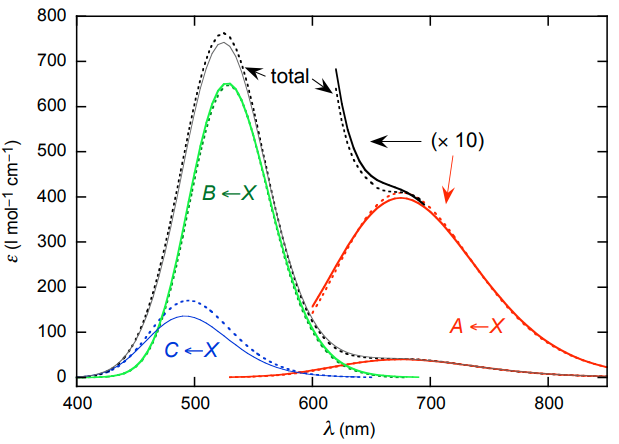
\includegraphics[width=0.9\textwidth]{graphics/literature-epsilon.png}
        \caption{Molar absorption coefficient $\varepsilon(\lambda)$ for molecular iodine at $T \approx \SI{35}{\celsius}$ \cite{tellinghuisen2011least}.}
        \label{fig:discussion:epsilon}
    \end{minipage}
    \hfill
     \begin{minipage}[b]{0.44\textwidth}
        \centering
        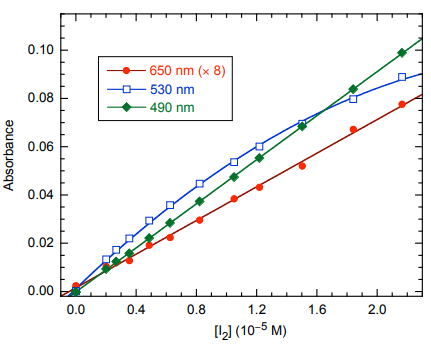
\includegraphics[width=0.9\textwidth]{graphics/literature-concentration.png}
        \caption{Absorbance $A(c)$ for molecular iodine at $T \approx \SI{35}{\celsius}$ \cite{tellinghuisen2011least}.}
        \label{fig:discussion:concentration}
    \end{minipage}
\end{figure}

The obtained concentrations $c$ for the single-pass configuration are therefore, at least with respect to orders of magnitude, assumed to be correct. However, for the triple-pass configuration at $T = \SI{53(3)}{\celsius}$, the obtained concentration amounts to $c = \SI{22(3)}{\milli\mol\per\m^3}$ as opposed to the corresponding single-pass value $c = \SI{11(3)}{\milli\mol\per\m^3}$.

This might - in addition to the reasons already mentioned in Section \ref{sec:discussion:iodine-absorbance} - be attributed to additional losses of intensity due to reflections and the increased number of cell wall passes the laser beam has to overcome in the triple-pass configuration.

To overcome this problem, it is advisable to not artificially extend the effective path-length of the laser beam in the iodine gas by use of mirrors, but to actually use dedicated iodine cells of matching length. Furthermore, it should be ensured the glass walls of the iodine cell only exhibit negligible interaction with the wavelengths of interest in order to not distort the measured transmitted intensity $I_t$. Alternatively, the absorbance of the glass walls could be determined in a separate experiment and then be compensated for in the evaluation. Also, the number of mirrors should not be changed between measurements to keep the intensity loss at the mirrors constant among different configurations.



